\documentclass[letter,12pt,english, final]{article}
\usepackage{mikkel}
\title{Author Attribution by $N$-Gram Analysis in Corpora with Brief Texts}
\author{Mikkel Kj�r Jensen}
\date{\today}
\begin{document}
\pagestyle{headings}
\maketitle
\abstract{
I evaluate a character-level $n$-gram based author attribution method by Peng et al. for attributing anonymous post on Danish Internet forums. I make an analysis of where and in which circumstances Author Attribution can, and cannot, be used on the Internet, and which test are relevant to gauge the effectiveness of the Internet based Author Attribution. I show that the the unmodified method with Good-Turing smoothing cannot be used to identify anonymous posts, and outline my thoughts on both the main problems, and what might be done to improve the method.}
\tableofcontents
\section{Introduction}
\label{introduction}
Authorship Attribution is the science of attributing the ownership of a disputed or anonymous text, given a list of potential authors. A corpora (a relevant subset of these authors texts) are then analysed, and the gained information is then used to find the most likely author of the disputed text.\\

The most famous case of Author Attribution is the attribution of 12 essays written in the \q{The Federalist Papers} series, whom both Alexander Hamilton and James Madison claimed to have written. Most modern Authorship Analysis believes that James Madison wrote them \cite{Fung03thedisputed}\fixme{Tentive: Is this good enough?}.\\
 The introduction of computers, and the Internet, where texts can be published anonymously, has increased the importance of Author Attribution, as it is now easier than ever before to commit plagiarism or illegal sharing of texts (such as for school projects). Author Attribution might also be used for the purpose of Internet related harassment, or inflammatory speech - thus circumventing the otherwise implicit anonymity found on the Internet \fixme{should it be here? Is it correctly worded}.\\ 

I will in this paper try to apply an already developed Author Attribution technique to posts found on Internet forums, and try to evaluate the quality of the result.\\

Internet forums are interesting to study, since the posts that comprise them are short, informal, and full of bad spelling and grammar\footnote{Not to mention the many strange abbreviations (``lol'', ``btw''), and features unique to the Internet (such as hyperlinks or embedded pictures)}. All of this quite unlike the works of famous authors (who tend to be used in the studies \cite{nr4}). 

\subsection{Scope and Limitations}
\label{scope}
A common feature in papers about Authorship Attribution is that their sample languages tend to be English, Greek and Chinese \cite{syntactic}, \cite{nr2}, \cite{nr4} and \cite{app-spe}. Since I do not have any relation to any Greek or Chinese forum, and indeed no ability to speak or understand either language, I have chosen to exclusively concentrate on forums and methods that works on a character based language - more specifically Danish.

\subsection{Expectations to the reader}
\label{expectations}
I expect the reader to be familiar with the problems within the field Author Attribution, as well as having a theoretical and practical experience with applying these techniques - especially the n-gram and statistical methods. Due to the nature of the sample content, it would be advisable if the reader has a familiarity with a cross section of relaxed non-formal Internet forums, and the kind of posts made on these. Sites such as Slashdot.org or a console gaming forum would be preferable.

\subsection{Learning targets and objectives}
\label{learning}
\subsubsection{Learning targets}
After having completed this assignment I will have learned 
\begin{itemize}
\item To briefly be able to summarise techniques, practical as well as theoretical, for authorship attribution.
\item Apply a simple technique for authorship attribution on a limited and specific domain with texts, which have special syntactical characteristics.
\item To be able to implement and test the above in a practical manner.
\item To be able to properly interpret these test results
\end{itemize}

\subsection{Reader guide}
In this section I give a quick overview of what the different section in report will cover.
\fixme{Final fixme: Make sure that it points to the correct sections}
\begin{description}
\item[Section \ref{introduction}] The introduction to the report, which will introduce the subject and explain my goals
\item[Section \ref{choiceMethod}] A survey of the different methods to do Author Attribution  
\item[Section \ref{method}] Explanation of the method used in my project
\item[Section \ref{consideration}] Considerations 
\item[Section \ref{tests}] Tests
\item[Section \ref{interpretation}] Interpretation of results
\item[Section \ref{conclusion}] The conclusion of the report, where I will sum up the findings  
\end{description}


\section{Various techniques used for Author attribution}
\label{choiceMethod}
I will in this section discuss the major different types of Author Attribution that exists, and debate the advantages and disadvantages of using each for this project.

To give an example of the different techniques, I will try to use a text extract from ``The Federalist Papers'' \cite{federalist} \footnote{To be more precise, the first essay (i.e. the lowest numbered one) that both Axelander Hamilton and James Madison have claimed to write} unless it is not applicative. It should be noted that each chosen method is merely an example for that category and should be seen as nothing more.

I will use the following criteria for judging the method's effectiveness:
\begin{itemize}
\item It should work on reasonably sized amount of text
\item The time complexity inherent in the algorithm should not be too large
\item I should be practically able to implement the solution without using an unreasonable amount of time
\item I should not be required to be an expert in natural language processing to be able to implement the solution
\item The solution should work on languages using a character alphabet, though it would be a plus if it could also be used on pictogram based languages.
\end{itemize}

\subsection{Example text}
The example text used will be:\\
\q{His proposition is, "that whenever any two of the three branches of government shall concur in opinion, each by the voices of two thirds of their whole number, that a convention is necessary for altering the constitution, or CORRECTING BREACHES OF IT, a convention shall be called for the purpose.}
From \cite{federalist}

\method{Character}
{\label{character}
Lexical analysis works on the character as the basic unit. I will here focus on n-gram analysis. N-gram analysis is done by taking a text, and breaking it into all possible permutations of n-consecutive ``grams''\footnote{A gram could, depending on the algorithm either be a word, character, or other subsection of the text.}. Once all the n-grams for a text have been computed, they are used in a statistical analysis with the corpora of the possible authors. 
}
{
I have in the following\footnote{Since any reasonable large text would create a very large number of 3-grams, I have chosen, unlike all the other examples, to use only the part before the first comma.} chosen to represent whitespace by the $\_$ character:
\q{His proposition is,}
which would create the following 3-grams: \ngr{His}, \ngr{is\_}, \ngr{s\_p}, \ngr{\_pr}, \ngr{pro}, \ngr{rop}, \ngr{opo}, \ngr{pos}, \ngr{osi}, \ngr{sit}, \ngr{iti}, \ngr{tio}, \ngr{ion}, \ngr{on\_}, \ngr{n\_i}, \ngr{\_is}, \ngr{is,}. 
}
{
\item Does not require specialised tools or much in the way prepossessing
\item Gives very good results in practice - see \cite{nr4} and \cite{nr3}.
\item The text does not need to be spelled correctly (as long as words are spelled consistently)
\item Ignores problems with word or sentence boundaries.
}
{
\item Can create very large data sets, since trying to create all n-grams on a text with m characters (given $n < m$) will result in m - n + 1 n-grams - each n characters - resulting in n * (m - n + 1) = n*m - $n^2$ + n characters.
\item Might not be applicable on alphabets based on symbols or pictogram's instead of individual letters (though it should avoid any word barrier problem - which is not a trivial problem in, for example Chinese\footnote{See \cite{nr1} p. 540}).
\item The statistical method might be very complex.
}

\method{Syntactic Features}
{\label{syntactic}
Methods that works on syntatic features tries to identify the author through the syntactic
features prevalent in the corpus of the authors
work. The underlying assumption is that each author has a certain way of writing, a style (which should be distinguished from the definition used in \ref{stylistic}), that they subconsciously in their text. Syntactic features include the frequency of different types of phrases (for instance \cite{style} uses concepts such as noun phrases, verb phrases, prepositional phrase, adverbial phrase and conjunctions\footnote{A naunphrase is a phrase that centers around a noun, while a verb phrase is a phrase that centers around a verb, and so on. A conjunction is a part of text that bridges two different parts, but has little meaning in itself}) and the frequency of punctuation.
} 
{
In the follow NP defines a Noun Phrase, VP a Verb Phrase, PP prepositional phrase, ADVP a adverbial phrase and CON conjunction.\\
\q{\ann{NP}{His proposition is}, "\ann{CON}{that whenever any two of \ann{NP}{the three branches of government} \ann{VP}{shall concur in opinion}, \ann{NP}{each by the voices of two thirds of their whole number}, \ann{NP}{that a convention is} \ann{VP}{necessary for altering the constitution},\ann{CON}{or CORRECTING BREACHES OF IT}, \ann{VP}{a convention shall be called for the purpose.}}
}
}
{
\item Could very well be very accurate.
}{
\item Requires advanced software that can identify the different parts of the sentence - which is beyond the scope of this project.

}

\method{Stylistic information}
{\label{stylistic}
Looking at the style of a text seems like an obvious choice when trying to identify the author (and indeed, not only the name, but also other data, like age and sex). In order to do, the text must be parsed to identify and mark parts of the text for certain predefined categories. \cite{style} mentions 3 top categories: 
\begin{description}
\item[Cohesion:] How a Text is constructed. Is constructed out of ``Elaboration'', ``Extension'' and ``Enhancement''.
\item[Assessment:] How a text \q{constructs propositions as statements of belief, obligation, or necessity}\footnote{\cite{style}, p. 804} - constructed out of  ``Type'', ``Value'', ``Orientation'', ``Objective'', ``Manifestation'', each with further subcategories, all hung on certain words.
\item[Appraisal:] Qualifiers
\end{description}
}
{
I have annotated the words that I believe might have been annotated by the system. However, I would like to note that this is only an approximation, and should not be taken as a qualification of the system described in \cite{style}:\\
\q{His proposition is, "that \ann{Value}{whenever} any two of the three branches of government shall concur in opinion, \ann{Elaboration}{each by the voices of two thirds of their whole number}, \ann{Orientation}{that a convention is necessary for altering the constitution, or CORRECTING BREACHES OF IT}, a convention \ann{Type}{shall} be called for the purpose.}
}  
{
\item Does not care about word or phrase boundaries.
\item Given that the system could differentiate between the different cases, it is likely that information about the text could be used to construct a profile.
}{
\item For optimal efficiency it would require the entire text to be spelled correctly. Since I intend to create my corpora from text from Internet forums - this requirement cannot be guarantied to be satisfied.
\item The system seems to require that the specific words must be identified and tied to categories. This would mean that it cannot be applied to another language without a prohibitively amount of work.
} 

\method{Application Specific}
{\label{application}
Instead of trying to fit a general model on on every text, the application specific takes care to use information about the medium in question - such as HTML tags for message on Internet forums, indentation, the use of signature, fonts, size etc.
}
{
\fixme{Find and add example}
Since this method is mainly for use for web based applications, I cannot use the example from the Federalist papers, and i will therefore use another example, that I have taken from the webpage [something]. 
\q{}
}
{
\item Might be applicable since this project this with Internet forums, which are known to use different structures when writing their posts.
\item Could very well improve the number of correctly attributed papers, as many forum regulars (who are the only ones that leave enough information to be identified) tend to have signatures and/or signature styles, as well as the use of links, bold and italic etc. .
}{
\item Might very well become too specific, and will thus only work on a subsection of forums or wikis (and not on those that have their own style or formatting).
\item Is described very vaguely - there is not much information on how the information should be processed or gathered (which in this case might be non-trivial).
\item Requires more advanced pattern recognition than could be implemented in this project. 
}

\subsection{Conclusion}
\label{technique:conclusion}
From this I have concluded that the best choice would be to use the character based n-gram approach - since it is both simpler and less labour intense than some of the other attribution models, while at the same time giving good results. Since the data I have to use is in Danish (and thus character based), I will not try to accommodate languages whose alphabet is pictogram based - e.g. Chinese.


\subsection{Choice of n-gram analysis}

\subsubsection{\cite{nr3}}
\cite{nr3} first selects the most important n-grams, using a number of rules (which, due to their complexity, will not be included here). In order to compare whether or not a certain author has written a certain text, another involved formula is then used, to gauge the information gain given the corpora of the author.

I find this n-gram analysis way of analysing intimidating - not only does the functions themselves seem rather advanced, but the ``out-sourcing'' of key concepts to other papers (which may contain even more implementation details is disturbing). Another problem is that the key glue function requires much manual tuning, which is language specific - which are one of the things I would like to avoid. 

\subsubsection{\cite{nr2}}
This paper uses a improved version of the algorithm found in \cite{Bennet}. \cite{Bennet} uses the basic idea that an authors profile can be found by calculating the difference between the frequency of a character in the English language (based on some standard frequency) and the frequency of the author.\\

The Authors of \cite{nr2}, however, use the following formula
$$
\sum_{n \in profile}\left(\frac{2 \cdot (f_1(n) - f_2(n))}{f_1(n) + f_2(n)}\right)^2
$$
which calculates the dissimilarity between the text t and one of the potential authors. $f_1(n)$ and $f_2(n)$ is the frequency of n-gram n in the document and the corpora of the author, respectively. 

This method has the clear advantage that it is rather straightforward, and unlike \cite{Bennet} it does not require standard frequencies for the English language (which there could be multiple versions off - and therefore lead to different results, depending on the version used).

\subsection{\cite{nr4}}
The method found in \cite{nr4} is a method based on statistical analysis, which implements its own algorithm to rate the similarity of the different authors. The underlying assumption is that the chance of the i'th gram being something is a function being based on all the i - 1 preceding grams. Since it is practically unfeasibly to base it on the i - 1 preceding grams, the implemented method only looks on the last n grams, where $n \in \{3,4,5,6 \}$. 

\subsection{Final choice}

In the end I choose \cite{nr4} for several reasons:
\begin{itemize}
\item The algorithm looked like it could be implemented without too much work
\item The authors had reported good results on the English language, as well as Chinese and Greek, which I presume would also mean good results for Danish.
\item The good results had been reported on famous Authors with a very specific way of writing - and the Authors themselves note that it would be interesting to apply their methods on less distinct corpora. 
\end{itemize}

\section{Method used}
\label{method}

\fixme{Make a proper introduction}
The method in \cite{4} tries to find the author with the greatest probability of having written a given text t. It does so by calculating the probability of each author having written the text, and then chooses the one with the greatest probability.

It should be mentioned that my implementation looks only on characters while the solution proposed in \cite{nr4} uses words\footnote{Thus the each ``gram'' would consist of a word}, which   \fixme{Should this be here? - should be in the report at all}.

The probability is calculated as follows:
\begin{enumerate}it be 
\item First an author a is chosen from the pool of A 
\item For each n-gram n in the text t we check to see whether the n-gram appears in the corpus of a
\begin{description}
\item[$n \in n-gram(a)$:] Return the result of probHat on n
\item[$n \notin n-gram(a)$:] Return the normalization\_constant(n) * probability($n^\prime$ - where $n^{\prime}$ is n with the first character removed (so if n =``abc'', then $n^{\prime}$ = ``bc'' 
\end{description} 
\end{enumerate}

In the following $c_n$ is the n'th character in the text. As stated in \cite{nr4}, the probability of the value of i'th character is based on the past i - 1 characters (with the more recent characters counting for more \fixme{is this true}). However, calculating this probability would be prohibitory expensive. With n-grams, we only use the probability for the last n characters - so the interesting characters would be $c_{i - n + 1} \ldots c_{i}$.

\begin{equation*}
Pr(c_{i - n + 1} \ldots c_{i}) = \left\{
\begin{array}{rl}
\hat{P}r(c_{i - n + 1} \ldots c_{i}), \text{if } \#(c_{i - n + 1} \ldots c_{i}) > 0\\
\beta(c_{i - n + 1} \ldots c_{i-1}) \cdot Pr(c_{i - n + 2} \ldots c_{i}), \mathrm{otherwise}
\end{array} \right.
\end{equation*}

where 
$$
\hat{P}r(c_{i - n + 1} \ldots c_{i}) = \frac{discount \#(c_{i - n + 1} \ldots c_{i})}{\#(c_{i - n + 1} \ldots c_{i-1})}
$$

$$
\beta(c_{i - n + 1} \ldots c_{i-1}) = 
\frac
{1 - \sum_{x \in (c_{i - n + 1} \ldots c_{i-1})}\hat{P}r(c_{i - n + 1} \ldots c_{i-1} x)}
{1 - \sum_{x \in (c_{i - n + 1} \ldots c_{i-1})}\hat{P}r(c_{i - n + 2} \ldots c_{i-1} x)}
$$
and 
$discount\#(c_{i - n + 1} \ldots c_{i})$ 
is the discounted probability, calculated by using Good-Turing smoothing\footnote{Which the report mentions gives good results in practice, as well as a fair speed \cite{nr4}}\fixme{Either refer to a source that describes Good-Turing smoothing or explain why it is needed} against the corpora for the author we are calculating against. The discounted smoothing is done to remove some of the n-grams that appears infrequently, and thus has no real significance for the corpora. This was especially relevant when the n-grams consited of words, as it did in \cite{nr4}, since the alfabet of words in the English language than the alfabet of letters, and thus would leave them with a too large dataset to shift through. \fixme{Decide whether it is worth explaining the division.}. The division of the number of occurences of $c_{i - n + 1} \ldots c_{i - 1}$ in the corpora is to make sure the  

%\fixme{Should this be here or moved up?}
%c_{i - n + 1} c_{i - n + 2} \ldots c_{i-1}

\section{Implementation}
\label{implementation}

In this section I will try to describe the implementation choices I have made in this project.

\subsection{Choice of programming language}
I choose to write my project in Python as I felt that a fast development time was more important than a super fast program.

\subsection{Creation of $n$-grams}
Since the creation of $n$-grams themselves was not a critical part of the project, I opted not to write my own code. Therefore I choose \texttt{python-ngram} (version 2.0b2) which can be found at http://python-ngram.sourceforge.net/\footnote{Address has been tested to work on the 13th of August, 2009}. I have made alterations to the program, the most important of which are the following:

\subsubsection*{Numbers}
Since numbers are bound to appear in some texts, I have chosen to represent them as the escape characters ``$\backslash$v'', since it is the appearance of numbers and their pattern that is interesting, not the numbers themselves.

\subsubsection*{Padding}
The code would originally add padding to the start and the end of the text. This was most likely done to ensure that the $(n-1)$ first and the $(n-1)$ last characters would have their own $n$-grams. However, since I also create 1 and 2 grams, this is not needed (see below).

\subsubsection*{Implementation changes}
Through experimentation, I have found that it essential to not only create the 3-grams, but also the 1- and 2- grams. If these $n$-grams are not created, then the probability of most the $n$-grams will be 0, just as what happened to $p_3$ in section \ref{Good-Turing}, p. \pageref{Good-Turing}.

\subsection{Good-Turing smoothing}
Like above, I did not choose to write my own Good-Turing smoothing, but have instead used the \texttt{Natural Language Toolkit} for python, version 0.9.9, which can be found at www.nltk.org\footnote{Address has been tested to work on 13th of August, 2009}.

\subsection{Scalability of implementation}
In order to measure whether or not the algorithm scales, I have found it necessary to make 2 separate tests: 
\begin{enumerate}
\item The time it takes to create the $n$-grams from the corpora. The only parameter in this case is the number of texts that appears in the corpora.
\item The time it takes to decide which author is most likely to have written a text. This test has 2 parameters: The number of texts in the corpora to test against, and the number of test to make
\end{enumerate}

In order to get a proper resolution for both tests, I have chosen 12 different corpora and text sizes, and have tested all $12 \times 12$ combinations. The numbers for both the corpora and the texts are as follows $100, 200, 300, \ldots, 1100, 1200$.\\

I ran the tests --- serially --- on a computer with a 8x3.06Ghz Core i7-950 with 6 GB of RAM, running Windows XP Pro. 

\subsubsection{Make $n$-gram}
\begin{tabular}{|c|c|c|c|c|c|c|}
\hline 
\# n-grams & 100& 200& 300& 400& 500& 600\\ 
\hline 
Time& 0.04700& 0.09300& 0.1410& 0.1870& 0.2650& 0.3290\\ 
\hline 
\end{tabular}
 
\begin{tabular}{|c|c|c|c|c|c|c|}
\hline 
\# n-grams & 700& 800& 900& 1000& 1100& 1200\\ 
\hline 
Time& 0.375& 0.4380& 0.5310& 0.5630& 0.6100& 0.6570\\ 
\hline 
\end{tabular}\\ \\

Both the above table and figure \ref{fig:ngram} clearly shows that the time required to make the $n$-grams grows liner with the number of posts in the corpora.

\begin{figure}[!hbp]
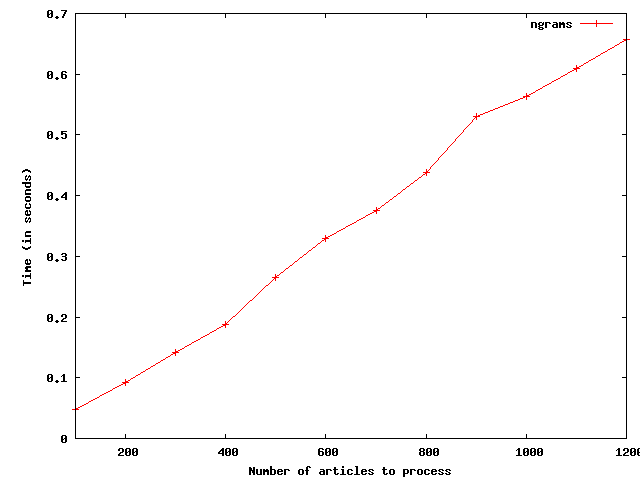
\includegraphics[width=\textwidth]{tabeller/ngram.png}\\
\caption{Time used to create $n$-grams compared to the number of texts in the corpora\label{fig:ngram}}
\end{figure}

\subsubsection{Decide authors}
The horizontal values are the number of texts in the corpora, while the vertical values are the amount of texts that have to be attributed.\\
\begin{tabular}{|c|c|c|c|c|c|c|c|c|c|c|c|c|c|}
\hline 
 & 100 & 200 & 300 & 400 & 500 & 600 & 700 & 800 & 900 & 1000 & 1100 & 1200\\ 
\hline 
100 & 55.20 & 79.24 & 100.7 & 113.7 & 127.7 & 138.9 & 152.2 & 160.5 & 170.3 & 184.5 & 193.5 & 203.4\\ 
\hline 
200 & 104.5 & 150.7 & 192.0 & 217.7 & 244.2 & 265.5 & 290.4 & 305.9 & 324.3 & 351.5 & 368.8 & 387.6\\ 
\hline 
300 & 158.7 & 229.2 & 292.7 & 330.7 & 371.3 & 403.5 & 440.8 & 464.3 & 491.9 & 533.0 & 559.0 & 587.3\\ 
\hline 
400 & 212.1 & 306.8 & 391.2 & 442.1 & 496.4 & 539.2 & 588.6 & 619.7 & 656.1 & 710.5 & 745.1 & 782.6\\ 
\hline 
500 & 279.5 & 403.9 & 514.4 & 581.0 & 652.2 & 708.1 & 772.3 & 812.6 & 860.2 & 933.9 & 981.1 & 1032\\ 
\hline 
600 & 344.3 & 497.8 & 634.8 & 717.2 & 805.7 & 874.8 & 954.2 & 1004 & 1062 & 1150 & 1206 & 1267\\ 
\hline 
700 & 385.2 & 559.0 & 713.5 & 806.1 & 905.5 & 983.0 & 1072 & 1128 & 1193 & 1292 & 1355 & 1423\\ 
\hline 
800 & 449.3 & 650.7 & 830.8 & 939.5 & 1056 & 1148 & 1253 & 1318 & 1394 & 1510 & 1583 & 1663\\ 
\hline 
900 & 521.9 & 755.8 & 965.6 & 1092 & 1228 & 1333 & 1454 & 1529 & 1618 & 1751 & 1837 & 1930\\ 
\hline 
1000 & 576.8 & 836.1 & 1068 & 1208 & 1359 & 1475 & 1619 & 1705 & 1807 & 1966 & 2069 & 2175\\ 
\hline 
1100 & 615.9 & 891.6 & 1136 & 1285 & 1541 & 1664 & 1808 & 1898 & 2004 & 2164 & 2263 & 2374\\ 
\hline 
1200 & 663.2 & 961.7 & 1227 & 1387 & 1559 & 1694 & 1848 & 1947 & 2060 & 2231 & 2340 & 2457\\ 
\hline 
\end{tabular}

Figure \ref{fig:work}, which is based on the 12th horizontal line\footnote{I have chosen this particular line, since it is the one that has to attribute all the authors, and thus would be the one that would best show if there was any significant non-linear time increase when the number of items in the corpora increased} (i.e. the bottom line in the table), clearly shows that the time required to attribute 1200 authors grows linearly with the amount of posts in the corpora.\\

Since both of these tests time consumption grows linearly with the number of texts in the corpora, it is clear that the algorithm could be used in practice, given that it is able to correctly attribute the authors  

\begin{figure}[!hbp]
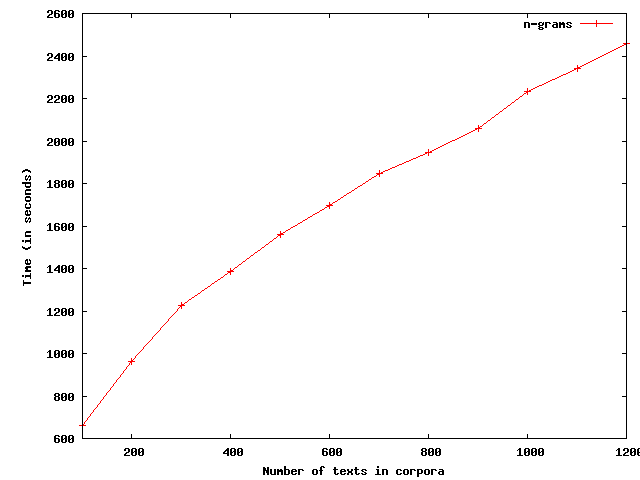
\includegraphics[width=\textwidth]{tabeller/work.png}
\caption{Time for text attribution with 1200 texts \label{fig:work}}
\end{figure}

\section{Considerations}
\label{considerations}

In this section I will describe the different tests that I will use to gauge the effectiveness of the algorithm. In order to do so probably I will perform each test multiple times (with multiple different texts) in order to gain a better overview of how effective the process is. Unless specifically noted I will run each test 3 times. \fixme{Should I test more times? Or should I perhaps mention the times I want to test locally at the different tests?}

\subsection{Initial smoke tests}
\label{smokeTest}
Some of the initial smoke tests showed some problems with the algorithm. 
One of the problems I found was that some shorter, bogus texts, would be given the greatest probability, even when the text in question was present in the corps that was analysed. A possible explanation for this is that the shorter text, has a greater probability for each word (and thus also for the \fixme{is this entire correct?} words that does not appear - as per Good-Turing smoothing).

\subsection{Limitations of the tests}
%In this study I have not been able to find texts from any of the authors from outside the source material that I have been working on. Therefore the only way

\test{
StressTest1
}{
Take a post from an author appearing in the corpora with a single, long text, and see if the author can be correctly attributed compared to the rest of the corpora.
}{
Check the limits of the algorithm. This is likely to fail.
}

\test{
StressTest2
}{
As above, but only against 100 posts
}{
Check the limits of the algorithm. This is likely to fail
}

\test{
StressTest3
}{
As above, but only against 10 posts
}{
Check the limits of the algorithm. This has a chance of succeding
}

\test{
StressTest4
}{
As above, but each author is only allowed one post.
}{
Check the limits of the algorithms. There is a non-trivial likelyhood that this will succeed.
}

\test{
ShortBogusTest
}{
Take a post from an author A with multiple long posts, and create a corpora with a short bogus post from a bogus author, together with real posts from A and others, and then try to see whether or not the bogus post is chosen
}{
A test to see whether the algorithm is suseptiable to give a heigher rank to posts with very little information (even if the bogus post is very dissimilar to the post that it is being cheked against)
}

\test{
Author10Post
}{
Take a post from an author A, who have written over 10 posts, and create a corpora with multiple long texts, including texts from author A. All authors must have written over 10 posts.
}{
A simple test to see whether the algorithm will work better on texts that are longer, and have authors who have written several posts
}

\test{
Author50Post
}{
Take a post from an author A, who have written over 50 posts, and create a corpora with multiple long texts, including texts from author A. All authors must have written over 50 posts.
}{
A simple test to see whether the algorithm will work better on texts that are longer, and have authors who have written many posts
}

%\test{
%Author100Post
%}{
%Take a post from an author A, who have written over 100 posts, and create a corpora with multiple long texts, including texts from author A. All authors must have written over 100 posts.
%}{
%A simple test to see whether the algorithm will work better on texts that are longer, and have authors who have written many posts
%}

\section{Tests}
\label{tests}

In this section present my test results in order to determine the effectiveness of my implementation.

In order to make my test results comparable with \cite{nr4} I will use the same parameters that they used. To make it easier to compare with the results in \cite{nr4}, I will keep all percentage results as a faction (e.g. 1 would be 100 \% and 0.33 would be 33 \%) --- results not computed in \cite{nr4} will however, be in percentage. These I will look for are: 

\begin{description}
\item[Overall Average] The number of correctly attributed texts divided by the number of texts that have been attributed. E.g. if 8 texts have been correctly attributed, and 10 texts have been attributed, then the overall average would be 0.8 

\item[Precision] The number of correctly attributed texts for an author, divided by the total number of texts that have been attributed to that author. E.g. if the author has had 8 texts correctly attributed to him, and in total 10 texts have been attributed to him, then the Precision would be 0.8. Thus, this is essentially local accuracy.

\item[Recall] Recall is the number of correctly attributed texts for an author, divided by the by the number of texts that should have been attributed to. E.g. if the authors has had 8 texts correctly attributed to him, but there was 10 texts there was to be attributed --- then the recall is 0.8.

\item[F-measure] F-measure is calculated like so: $\frac{2 \times precision \times recall}{precision+recall}$ 

\item[Macro-average F-measure] The Macro-average F-measure is the average of all the authors F-measure. 
\end{description}

\subsection{Random selection}
In order to have a baseline to compare my results against, I have for each subtest made a random selection test. For each text that had to be selected in the test, I have selected one million random authors as the texts author. The result of this will be presented at the end of each subsection, and will be compared to the real results in section \ref{interpretation}. If the random selection returns better results than the method found in \cite{nr4}, then my implementation of \cite{nr4} cannot be used. 

Since I do a million random selections, the concept of precision will become meaningless in tests when there is only text from one author --- since there in practice is no chance of that author not being chosen once. I will therefore only show precision for Random selection tests when there are multiple authors. 

The code that generates the random selections can be found in section \ref{code:randomTest}.

\subsection*{Key}
In the following I each author will follow the following format: Axx$^{n}$, where xx is the number identifying the author, and n is the number of posts that the author has written. Furthermore, since no test contain every author, the authors who appear both in the corpus and the texts that are to be attributed will have the following formatting: \aAuthor{Axx$^{n}$}, whereas authors who only appear in the corpus will have no such formatting. All authors who have written only 1 post, will furthermore have the following formatting: \veryFew{Axx$^{n}$}. These formatting may overlap.\\

\subsection{Test results}

\subsubsection{StressTest1}
A single post is compared against the entire corpus --- for more information, \nref{StressTest1}.\nl

\begin{tabular}{|c||c|c||c|}
\hline 
\multicolumn{4}{|c|}{Computer Estimate}\\
\hline 
True Label & \aAuthor{A4}$^{137}$ & \veryFew{A66}$^{1}$ & Recall \\
\hline 
\aAuthor{A4}$^{137}$ &  & 1 &  0.0\\
\veryFew{A66}$^{1}$ &  &  &  0.0\\
\hline 
Precision & 0.0 & 0.0 & \\
\hline 
\multicolumn{4}{|c|}{Overall Accuracy: 0 Macro-average F-measure: 0.0}\\
\hline 
\end{tabular} 
\nl

\begin{tabular}{|c||c|c||c|}
\hline 
\multicolumn{4}{|c|}{Computer Estimate}\\
\hline 
True Label & \aAuthor{A38}$^{5}$ & \veryFew{A61}$^{1}$ & Recall \\
\hline 
\aAuthor{A38}$^{5}$ &  & 1 &  0.0\\
\veryFew{A61}$^{1}$ &  &  &  0.0\\
\hline 
Precision & 0.0 & 0.0 & \\
\hline 
\multicolumn{4}{|c|}{Overall Accuracy: 0 Macro-average F-measure: 0.0}\\
\hline 
\end{tabular} 
\nl

\begin{tabular}{|c||c|c||c|}
\hline 
\multicolumn{4}{|c|}{Computer Estimate}\\
\hline 
True Label & \veryFew{A50}$^{1}$ & \aAuthor{A65}$^{10}$ & Recall \\
\hline 
\veryFew{A50}$^{1}$ &  &  &  0.0\\
\aAuthor{A65}$^{10}$ & 1 &  &  0.0\\
\hline 
Precision & 0.0 & 0.0 & \\
\hline 
\multicolumn{4}{|c|}{Overall Accuracy: 0 Macro-average F-measure: 0.0}\\
\hline 
\end{tabular} 
\nl

\texttt{Random selection:}\nl
\begin{tabular}{|c|c|c|c|}
\hline 
Name & Recall &  Hits & Miss \\ 
\hline 
\aAuthor{A4$^{137}$} & 0.10 & 0.10 & 0.0 \\ 
\hline 
\multicolumn{4}{|c|}{Overall Accuracy: 0.104  Macro-average F-measure: 0.188 }\\ 
\hline 
\end{tabular}

\subsubsection{StressTest2}
A single post from an author who has written \postAmount{Some} posts are checked against the entire corpus, \nref{StressTest2}.\\

\texttt{Stress Test 2.1:}\nl
\begin{tabular}{|c||c||c|}
\hline 
\multicolumn{3}{|c|}{Computer Estimate}\\
\hline 
True Label & A4 & Recall \\
\hline 
A4 & 1 &  0.00\\
\hline 
Precision & 1.0 & \\
\hline 
\multicolumn{3}{|c|}{Overall Accuracy: 1.0 Macro-average F-measure: 0.333333333333}\\
\hline 
\end{tabular} 
\nl

\texttt{Stress Test 2.2:}\nl
\begin{tabular}{|c||c|c||c|}
\hline 
\multicolumn{4}{|c|}{Computer Estimate}\\
\hline 
True Label & \aAuthor{A0}$^{75}$ & A24$^{71}$ & Recall \\
\hline 
\aAuthor{A0}$^{75}$ &  & 1 &  0.0\\
A24$^{71}$ &  &  &  0.0\\
\hline 
Precision & 0.0 & 0.0 & \\
\hline 
\multicolumn{4}{|c|}{Overall Accuracy: 0 Macro-average F-measure: 0.0}\\
\hline 
\end{tabular} 
\nl

\texttt{Stress Test 2.3:}\nl
\begin{tabular}{|c||c|c||c|}
\hline 
\multicolumn{4}{|c|}{Computer Estimate}\\
\hline 
True Label & A24 & \aAuthor{A65} & Recall \\
\hline 
A24 &  &  &  0.00\\
\aAuthor{A65} & 1 &  &  0.0\\
\hline 
Precision & 0.0 & 0 & \\
\hline 
\multicolumn{4}{|c|}{Overall Accuracy: 0 Macro-average F-measure: 0}\\
\hline 
\end{tabular} 
\nl

\texttt{Random selection:}\nl
\begin{tabular}{|c|c|c|c|}
\hline 
Name & Recall &  Hits & Miss \\ 
\hline 
\aAuthor{A13$^{82}$} & 0.19 & 0.19 & 0.0 \\ 
\hline 
\multicolumn{4}{|c|}{Overall Accuracy: 0.19  Macro-average F-measure: 0.32 }\\ 
\hline 
\end{tabular}

\subsubsection{StressTest3}
One post from an author who has written \postAmount{Many} posts are checked against the entire corpus, \nref{StressTest4}.\\

\texttt{Stress Test 3.1:}\nl
\begin{tabular}{|c||c|c||c|}
\hline 
\multicolumn{4}{|c|}{Computer Estimate}\\
\hline 
True Label & A1$^{105}$ & \aAuthor{A35}$^{119}$ & Recall \\
\hline 
A1$^{105}$ &  &  &  0.0\\
\aAuthor{A35}$^{119}$ & 1 &  &  0.0\\
\hline 
Precision & 0.0 & 0.0 & \\
\hline 
\multicolumn{4}{|c|}{Overall Accuracy: 0 Macro-average F-measure: 0.0}\\
\hline 
\end{tabular} 
\nl

\texttt{Stress Test 3.2:}\nl
\begin{tabular}{|c||c|c||c|}
\hline 
\multicolumn{4}{|c|}{Computer Estimate}\\
\hline 
True Label & A1 & \aAuthor{A38} & Recall \\
\hline 
A1 &  &  &  0.00\\
\aAuthor{A38} & 1 &  &  0.0\\
\hline 
Precision & 0.0 & 0 & \\
\hline 
\multicolumn{4}{|c|}{Overall Accuracy: 0 Macro-average F-measure: 0}\\
\hline 
\end{tabular} 
\nl

\texttt{Stress Test 3.3:}\nl
\begin{tabular}{|c||c|c||c|}
\hline 
\multicolumn{4}{|c|}{Computer Estimate}\\
\hline 
True Label & A1 & \aAuthor{A65} & Recall \\
\hline 
A1 &  &  &  0.00\\
\aAuthor{A65} & 1 &  &  0.0\\
\hline 
Precision & 0.0 & 0 & \\
\hline 
\multicolumn{4}{|c|}{Overall Accuracy: 0 Macro-average F-measure: 0}\\
\hline 
\end{tabular} 
\nl

\texttt{Random selection:}\nl
\begin{tabular}{|c|c|c|c|c||c|c|c|c|c|}
\hline 
Name & Recall & Precision & Hits & Miss &Name & Recall & Precision & Hits & Miss \\ 
\hline 
A1$^{105}$ & 0.0 & 0 & 0 & 0.290111 & A4$^{137}$ & 0.0 & 0 & 0 & 0.379568 \\ 
\hline 
\multicolumn{10}{|c|}{Overall Accuracy: 0.33 Macro-average F-measure: 0.51}\\ 
\multicolumn{10}{|c|}{Total number of posts attributed to authors with less than 1 posts: 0}\\ 
\multicolumn{10}{|c|}{Percentage of posts attributed authors with 1 post: 0.0\%}\\ 
\hline 
\end{tabular}

\subsubsection{StressTest4}
A single text from an author is checked against all the texts, \nref{StressTest4} .\\

\texttt{Stress Test 4.1:}\nl
\begin{tabular}{|c||c|c||c|}
\hline 
\multicolumn{4}{|c|}{Computer Estimate}\\
\hline 
True Label & \veryFew{\aAuthor{A4}}$^{1}$ & \veryFew{A40}$^{1}$ & Recall \\
\hline 
\veryFew{\aAuthor{A4}}$^{1}$ &  & 1 &  0.0\\
\veryFew{A40}$^{1}$ &  &  &  0.0\\
\hline 
Precision & 0.0 & 0.0 & \\
\hline 
\multicolumn{4}{|c|}{Overall Accuracy: 0 Macro-average F-measure: 0.0}\\
\hline 
\end{tabular} 
\nl

\texttt{Stress Test 4.2:}\nl
\begin{tabular}{|c||c|c||c|}
\hline 
\multicolumn{4}{|c|}{Computer Estimate}\\
\hline 
True Label & \veryFew{\aAuthor{A38}}$^{1}$ & \veryFew{A65}$^{1}$ & Recall \\
\hline 
\veryFew{\aAuthor{A38}}$^{1}$ &  & 1 &  0.0\\
\veryFew{A65}$^{1}$ &  &  &  0.0\\
\hline 
Precision & 0.0 & 0.0 & \\
\hline 
\multicolumn{4}{|c|}{Overall Accuracy: 0 Macro-average F-measure: 0.0}\\
\hline 
\end{tabular} 
\nl

\texttt{Stress Test 4.3:}\nl
\begin{tabular}{|c||c|c||c|}
\hline 
\multicolumn{4}{|c|}{Computer Estimate}\\
\hline 
True Label & A32 & \aAuthor{A65} & Recall \\
\hline 
A32 &  &  &  0.00\\
\aAuthor{A65} & 1 &  &  0.0\\
\hline 
Precision & 0.0 & 0 & \\
\hline 
\multicolumn{4}{|c|}{Overall Accuracy: 0 Macro-average F-measure: 0}\\
\hline 
\end{tabular} 
\nl

\texttt{Random selection:}\nl
\begin{tabular}{|c|c|c|c|c||c|c|c|c|c|}
\hline 
Name & Recall & Precision & Hits & Miss &Name & Recall & Precision & Hits & Miss \\ 
\hline 
\veryFew{A0$^{1}$} & 0.0 & 0 & 0 & 0.011011 & \veryFew{A1$^{1}$} & 0.0 & 0 & 0 & 0.011087 \\ 
\hline 
\multicolumn{10}{|c|}{Overall Accuracy: 0.011 Macro-average F-measure: 0.022}\\ 
\multicolumn{10}{|c|}{Total number of posts attributed to authors with less than 1 posts: 0.022098}\\ 
\multicolumn{10}{|c|}{Percentage of posts attributed authors with 1 post: 100.0\%}\\ 
\hline 
\end{tabular}

\subsubsection{AuthorSomePost}
All the posts from a random author who has written \postAmount{Some} posts is checked against all the posts from all authors who have written \postAmount{Some} posts \nref{AuthorSomePost}.\\  

\texttt{AuthorSomePost 1:}\nl
\begin{tabular}{|c||c|c||c|}
\hline 
\multicolumn{4}{|c|}{Computer Estimate}\\
\hline 
True Label & \aAuthor{A0} & A24 & Recall \\
\hline 
\aAuthor{A0} &  & 75 &  0.0\\
A24 &  &  &  0.00\\
\hline 
Precision & 0 & 0.0 & \\
\hline 
\multicolumn{4}{|c|}{Overall Accuracy: 0 Macro-average F-measure: 0}\\
\hline 
\end{tabular} 
\nl

\texttt{AuthorSomePost 2:}\nl
\begin{tabular}{|c||c|c|c||c|}
\hline 
\multicolumn{5}{|c|}{Computer Estimate}\\
\hline 
True Label & \aAuthor{A2} & A24 & A3 & Recall \\
\hline 
\aAuthor{A2} &  & 97 & 1 &  0.0\\
A24 &  &  &  &  0.00\\
A3 &  &  &  &  0.00\\
\hline 
Precision & 0 & 0.0 & 0.0 & \\
\hline 
\multicolumn{5}{|c|}{Overall Accuracy: 0 Macro-average F-measure: 0}\\
\hline 
\end{tabular} 
\nl

\texttt{AuthorSomePost 3:}\nl
\begin{tabular}{|c||c|c|c||c|}
\hline 
\multicolumn{5}{|c|}{Computer Estimate}\\
\hline 
True Label & \aAuthor{A3}$^{99}$ & A13$^{82}$ & A24$^{71}$ & Recall \\
\hline 
\aAuthor{A3}$^{99}$ & 1 & 1 & 97 &  0.010\\
A13$^{82}$ &  &  &  &  0.0\\
A24$^{71}$ &  &  &  &  0.0\\
\hline 
Precision & 1 & 0.0 & 0.0 & \\
\hline 
\multicolumn{5}{|c|}{Overall Accuracy: 0.010 Macro-average F-measure: 0.02}\\
\hline 
\end{tabular} 
\nl

\texttt{Random selection:}\nl
\begin{tabular}{|c|c|c|c|c||c|c|c|c|c|}
\hline 
Name & Recall & Precision & Hits & Miss &Name & Recall & Precision & Hits & Miss \\ 
\hline 
\aAuthor{A0$^{75}$} & 0.18 & 1.0 & 13.241624 & 0.0 & A2$^{98}$ & 0.0 & 0 & 0 & 17.290265 \\ 
\hline 
\multicolumn{10}{|c|}{Overall Accuracy: 0.18 Macro-average F-measure: 0.3}\\ 
\multicolumn{10}{|c|}{Total number of posts attributed to authors with less than 1 posts: 0}\\ 
\multicolumn{10}{|c|}{Percentage of posts attributed authors with 1 post: 0.0\%}\\ 
\hline 
\end{tabular}

\subsubsection{AuthorManyPost}
All the posts from a random author who has written \postAmount{Many} posts is checked against all the posts from all authors who have written \postAmount{Many} posts \nref{AuthorManyPost}.\\  

\texttt{AuthorManyPost 1:}\nl
\begin{tabular}{|c||c|c|c||c|}
\hline 
\multicolumn{5}{|c|}{Computer Estimate}\\
\hline 
True Label & A1$^{105}$ & A4$^{137}$ & \aAuthor{A35}$^{119}$ & Recall \\
\hline 
A1$^{105}$ &  &  &  &  0.0\\
A4$^{137}$ &  &  &  &  0.0\\
\aAuthor{A35}$^{119}$ & 115 & 1 & 3 &  0.025\\
\hline 
Precision & 0.0 & 0.0 & 1 & \\
\hline 
\multicolumn{5}{|c|}{Overall Accuracy: 0.025 Macro-average F-measure: 0.05}\\
\hline 
\end{tabular} 
\nl

\texttt{AuthorManyPost 2:}\nl
\begin{tabular}{|c||c|c||c|}
\hline 
\multicolumn{4}{|c|}{Computer Estimate}\\
\hline 
True Label & A1$^{105}$ & \aAuthor{A4}$^{137}$ & Recall \\
\hline 
A1$^{105}$ &  &  &  0.0\\
\aAuthor{A4}$^{137}$ & 88 & 49 &  0.36\\
\hline 
Precision & 0.0 & 1 & \\
\hline 
\multicolumn{4}{|c|}{Overall Accuracy: 0.36 Macro-average F-measure: 0.51}\\
\hline 
\end{tabular} 
\nl

\texttt{AuthorManyPost 3:}\nl
\begin{tabular}{|c||c|c||c|}
\hline 
\multicolumn{4}{|c|}{Computer Estimate}\\
\hline 
True Label & \aAuthor{A1} & A4 & Recall \\
\hline 
\aAuthor{A1} & 101 & 4 &  0.96\\
A4 &  &  &  0.00\\
\hline 
Precision & 1.0 & 0.0 & \\
\hline 
\multicolumn{4}{|c|}{Overall Accuracy: 0.96 Macro-average F-measure: 0.95}\\
\hline 
\end{tabular} 
\nl

\texttt{Random selection:}\nl
\begin{tabular}{|c|c|c|c|c||c|c|c|c|c|}
\hline 
Name & Recall & Precision & Hits & Miss &Name & Recall & Precision & Hits & Miss \\ 
\hline 
A1$^{105}$ & 0.0 & 0 & 0 & 34.61188 & A4$^{137}$ & 0.0 & 0 & 0 & 45.156783 \\ 
\hline 
\multicolumn{10}{|c|}{Overall Accuracy: 0.33 Macro-average F-measure: 0.51}\\ 
\multicolumn{10}{|c|}{Total number of posts attributed to authors with less than 1 posts: 0}\\ 
\multicolumn{10}{|c|}{Percentage of posts attributed authors with 1 post: 0.0\%}\\ 
\hline 
\end{tabular}

\subsubsection{ShortBogusTest}
All texts from an author are tested against a corpus comprising only of the authors text, and 2 short bogus texts, in order to whether authors with few texts are given a too large probability when tested against. \pref{ShortBogusTest}

\texttt{Short Bogus Test 1:}\nl
\begin{tabular}{|c||c|c||c|}
\hline 
\multicolumn{4}{|c|}{Computer Estimate}\\
\hline 
True Label & A35 & Bogus & Recall \\
\hline 
A35 &  & 1 &  0.0\\
Bogus &  &  &  0.00\\
\hline 
Precision & 0.0 & 0.0 & \\
\hline 
\multicolumn{4}{|c|}{Overall Accuracy: 0.0 Macro-average F-measure: 0.0}\\
\hline 
\end{tabular} 
\nl

\texttt{Short Bogus Test 2:}\nl
\begin{tabular}{|c||c|c||c|}
\hline 
\multicolumn{4}{|c|}{Computer Estimate}\\
\hline 
True Label & A4 & Bogus & Recall \\
\hline 
A4 &  & 1 &  0.0\\
Bogus &  &  &  0.00\\
\hline 
Precision & 0.0 & 0.0 & \\
\hline 
\multicolumn{4}{|c|}{Overall Accuracy: 0.0 Macro-average F-measure: 0.0}\\
\hline 
\end{tabular} 
\nl

\texttt{Short Bogus Test 3:}\nl
\begin{tabular}{|c||c|c||c|}
\hline 
\multicolumn{4}{|c|}{Computer Estimate}\\
\hline 
True Label & \aAuthor{A1}$^{105}$ & Bogus$^{2}$ & Recall \\
\hline 
\aAuthor{A1}$^{105}$ &  & 1 &  0.0\\
Bogus$^{2}$ &  &  &  0.0\\
\hline 
Precision & 0.0 & 0.0 & \\
\hline 
\multicolumn{4}{|c|}{Overall Accuracy: 0 Macro-average F-measure: 0.0}\\
\hline 
\end{tabular} 
\nl

\texttt{Random selection:}\nl
\begin{tabular}{|c|c|c|c|}
\hline 
Name & Recall &  Hits & Miss \\ 
\hline 
\aAuthor{A35$^{119}$} & 0.98 & 0.98 & 0.0 \\ 
\hline 
\multicolumn{4}{|c|}{Overall Accuracy: 0.98  Macro-average F-measure: 1.0 }\\ 
\hline 
\end{tabular}

\subsubsection{UltimateStressTest}
A random half of the corpus is checked against the entire corpus, \nref{UltimateStressTest}.\\
Due to the size of the table, I have chosen to not represent the table in the manner used in \cite{nr4}, but instead just summing up the recall, precision, hits, misses (the number texts wrongly attributed the author), the number and percentage of texts attributed to an author with only 1 post.
\clearpage
\texttt{Ultimate Test 1:}\nl
\begin{tabular}{|c||c|c|c|c|c|c|c|c|c|c|c|c|c|c|c|c|c|c|c|c|c|c|c|c|c|c|c|c|c|c|c|c|c|c|c|c|c|c|c|c|c|c|c|c|c|c|c|c|c|c||c|}
\hline 
\multicolumn{52}{|c|}{Computer Estimate}\\
\hline 
True Label & \aAuthor{A0} & \aAuthor{A10} & \aAuthor{A11} & \aAuthor{A12} & \aAuthor{A13} & \aAuthor{A14} & \aAuthor{A15} & \aAuthor{A16} & \aAuthor{A17} & \aAuthor{A20} & \aAuthor{A26} & \aAuthor{A3} & \aAuthor{A30} & \aAuthor{A33} & \aAuthor{A34} & \aAuthor{A35} & \aAuthor{A36} & \aAuthor{A4} & \aAuthor{A40} & \aAuthor{A44} & \aAuthor{A46} & \aAuthor{A49} & \aAuthor{A50} & \aAuthor{A51} & \aAuthor{A52} & \aAuthor{A57} & \aAuthor{A58} & \aAuthor{A6} & \aAuthor{A60} & A61 & A62 & \aAuthor{A65} & A66 & \aAuthor{A67} & A68 & \aAuthor{A69} & A7 & \aAuthor{A72} & \aAuthor{A73} & \aAuthor{A74} & \aAuthor{A75} & \aAuthor{A77} & \aAuthor{A78} & A79 & \aAuthor{A80} & \aAuthor{A81} & \aAuthor{A83} & \aAuthor{A86} & A88 & \aAuthor{A89} & Recall \\
\hline 
\aAuthor{A0} &  &  &  &  &  &  &  &  &  &  &  &  &  &  &  &  & 7 &  &  &  &  &  & 6 &  &  &  &  &  &  & 51 &  &  & 5 &  & 1 &  &  &  &  &  &  &  &  &  &  &  &  &  & 1 & 4 &  0.0\\
\aAuthor{A10} &  &  &  &  &  &  &  &  &  &  &  &  &  &  &  &  & 1 &  &  &  &  &  & 1 &  &  &  &  &  &  & 2 &  &  &  &  &  &  &  &  &  &  &  &  &  &  &  &  &  &  &  &  &  0.0\\
\aAuthor{A11} &  &  &  &  &  &  &  &  &  &  &  &  &  &  &  &  & 1 &  &  &  &  &  &  &  &  &  &  &  &  & 4 &  &  &  &  & 1 &  &  &  &  &  &  &  &  &  &  &  &  &  &  &  &  0.0\\
\aAuthor{A12} &  &  &  &  &  &  &  &  &  &  &  &  &  &  &  &  & 2 &  &  &  &  &  &  &  &  &  &  &  &  & 5 &  &  & 3 &  &  &  &  &  &  &  &  &  & 1 &  &  &  &  &  & 1 &  &  0.0\\
\aAuthor{A13} &  &  &  &  &  &  &  &  &  &  &  &  &  &  &  &  & 11 &  &  &  &  &  & 4 &  &  &  &  &  &  & 37 & 1 &  & 9 &  & 7 &  &  &  & 2 &  &  &  &  &  &  &  &  &  & 5 & 6 &  0.0\\
\aAuthor{A14} &  &  &  &  &  &  &  &  &  &  &  &  &  &  &  &  &  &  &  &  &  &  &  &  &  &  &  &  &  & 1 &  &  &  &  &  &  &  &  &  &  &  &  &  &  &  &  &  &  &  &  &  0.0\\
\aAuthor{A15} &  &  &  &  &  &  &  &  &  &  &  &  &  &  &  &  &  &  &  &  &  &  & 1 &  &  &  &  &  &  &  &  &  &  &  &  &  &  &  &  &  &  &  &  &  &  &  &  &  &  &  &  0.0\\
\aAuthor{A16} &  &  &  &  &  &  &  &  &  &  &  &  &  &  &  &  &  &  &  &  &  &  &  &  &  &  &  &  &  & 1 &  &  & 2 &  &  &  &  &  &  &  &  &  &  &  &  &  &  &  &  &  &  0.0\\
\aAuthor{A17} &  &  &  &  &  &  &  &  & 1 &  &  &  &  &  &  &  &  &  &  &  &  &  &  &  &  &  &  &  &  &  &  &  &  &  &  &  &  &  &  &  &  &  &  &  &  &  &  &  &  &  &  1\\
\aAuthor{A20} &  &  &  &  &  &  &  &  &  &  &  &  &  &  &  &  & 3 &  &  &  &  &  &  &  &  &  &  &  &  & 9 & 1 &  &  &  &  &  &  &  &  &  &  &  &  &  &  &  &  &  & 1 & 1 &  0.0\\
\aAuthor{A26} &  &  &  &  &  &  &  &  &  &  &  &  &  &  &  &  & 1 &  &  &  &  &  & 3 &  &  &  &  &  &  & 2 &  &  & 1 &  & 1 &  &  &  &  &  &  &  &  &  &  &  &  &  &  &  &  0.0\\
\aAuthor{A3} &  &  &  &  &  &  &  &  & 1 &  &  &  &  &  &  &  & 15 &  &  &  &  &  & 7 &  &  &  &  &  &  & 41 & 1 &  & 4 &  & 18 &  & 1 &  &  &  &  &  &  &  &  &  &  &  & 2 & 9 &  0.0\\
\aAuthor{A30} &  &  &  &  &  &  &  &  & 1 &  &  &  &  &  &  &  & 1 &  &  &  &  &  & 4 &  &  & 1 &  &  &  & 6 & 1 &  & 4 &  & 2 &  &  &  & 1 &  &  &  &  &  &  &  &  &  & 1 & 3 &  0.0\\
\aAuthor{A33} &  &  &  &  &  &  &  &  &  &  &  &  &  &  &  &  &  &  &  &  &  &  &  &  &  &  &  &  &  & 1 &  &  &  &  &  &  &  &  &  &  &  &  &  &  &  &  &  &  &  &  &  0.0\\
\aAuthor{A34} &  &  &  &  &  &  &  &  &  &  &  &  &  &  &  &  & 1 &  &  &  &  &  &  &  &  &  &  &  &  & 3 &  &  &  &  &  &  &  &  &  &  &  &  &  &  &  &  &  &  &  &  &  0.0\\
\aAuthor{A35} &  &  &  &  &  &  &  &  &  &  &  &  &  &  &  &  & 19 &  &  &  &  &  & 6 &  &  &  &  &  &  & 67 & 1 &  & 2 &  & 7 &  &  &  & 1 &  &  &  & 8 &  &  &  &  &  & 1 & 7 &  0.0\\
\aAuthor{A36} &  &  &  &  &  &  &  &  &  &  &  &  &  &  &  &  & 1 &  &  &  &  &  &  &  &  &  &  &  &  &  &  &  &  &  &  &  &  &  &  &  &  &  &  &  &  &  &  &  &  &  &  1\\
\aAuthor{A4} &  &  &  &  &  &  &  &  &  &  &  &  &  &  &  &  & 11 &  &  &  &  &  & 18 &  &  & 2 &  &  &  & 48 & 1 &  & 28 &  & 8 &  &  &  &  &  &  &  & 12 &  &  &  &  &  & 3 & 6 &  0.0\\
\aAuthor{A40} &  &  &  &  &  &  &  &  &  &  &  &  &  &  &  &  & 1 &  &  &  &  &  & 1 &  &  &  &  &  &  & 1 &  &  &  &  & 1 &  &  &  &  &  &  &  &  &  &  &  &  &  &  &  &  0.0\\
\aAuthor{A44} &  &  &  &  &  &  &  &  &  &  &  &  &  &  &  &  &  &  &  &  &  &  &  &  &  &  &  &  &  & 2 &  &  &  &  &  &  &  &  &  &  &  &  &  &  &  &  &  &  &  &  &  0.0\\
\aAuthor{A46} &  &  &  &  &  &  &  &  &  &  &  &  &  &  &  &  &  &  &  &  &  &  &  &  &  &  &  &  &  &  &  &  &  &  &  &  &  &  &  &  &  &  &  & 1 &  &  &  &  &  &  &  0.0\\
\aAuthor{A49} &  &  &  &  &  &  &  &  &  &  &  &  &  &  &  &  &  &  &  &  &  &  &  &  &  &  &  &  &  & 2 &  &  &  &  &  &  &  &  &  &  &  &  &  &  &  &  &  &  &  &  &  0.0\\
\aAuthor{A50} &  &  &  &  &  &  &  &  &  &  &  &  &  &  &  &  &  &  &  &  &  &  & 1 &  &  &  &  &  &  &  &  &  &  &  &  &  &  &  &  &  &  &  &  &  &  &  &  &  &  &  &  1\\
\aAuthor{A51} &  &  &  &  &  &  &  &  &  &  &  &  &  &  &  &  &  &  &  &  &  &  &  &  &  &  &  &  &  & 2 &  &  &  &  &  &  &  &  &  &  &  &  &  &  &  &  &  &  & 1 &  &  0.0\\
\aAuthor{A52} &  &  &  &  &  &  &  &  &  &  &  &  &  &  &  &  & 5 &  &  &  &  &  & 1 &  &  & 1 &  &  &  & 10 &  &  & 3 &  & 6 &  & 1 &  &  &  &  &  &  &  &  &  &  &  &  & 1 &  0.0\\
\aAuthor{A57} &  &  &  &  &  &  &  &  &  &  &  &  &  &  &  &  &  &  &  &  &  &  &  &  &  & 2 &  &  &  &  &  &  &  &  &  &  &  &  &  &  &  &  &  &  &  &  &  &  &  &  &  1\\
\aAuthor{A58} &  &  &  &  &  &  &  &  &  &  &  &  &  &  &  &  & 3 &  &  &  &  &  &  &  &  &  &  &  &  & 2 & 1 &  &  &  & 2 &  &  &  &  &  &  &  &  &  &  &  &  &  & 2 & 2 &  0.0\\
\aAuthor{A6} &  &  &  &  &  &  &  &  &  &  &  &  &  &  &  &  &  &  &  &  &  &  & 2 &  &  &  &  &  &  & 2 &  &  &  &  & 1 &  &  &  &  &  &  &  &  &  &  &  &  &  &  & 1 &  0.0\\
\aAuthor{A60} &  &  &  &  &  &  &  &  &  &  &  &  &  &  &  &  &  &  &  &  &  &  &  &  &  &  &  &  &  & 2 & 1 &  &  &  &  &  &  &  &  &  &  &  &  &  &  &  &  &  &  &  &  0.0\\
A61 &  &  &  &  &  &  &  &  &  &  &  &  &  &  &  &  &  &  &  &  &  &  &  &  &  &  &  &  &  &  &  &  &  &  &  &  &  &  &  &  &  &  &  &  &  &  &  &  &  &  &  0.00\\
A62 &  &  &  &  &  &  &  &  &  &  &  &  &  &  &  &  &  &  &  &  &  &  &  &  &  &  &  &  &  &  &  &  &  &  &  &  &  &  &  &  &  &  &  &  &  &  &  &  &  &  &  0.00\\
\aAuthor{A65} &  &  &  &  &  &  &  &  &  &  &  &  &  &  &  &  & 2 &  &  &  &  &  &  &  &  &  &  &  &  & 5 &  &  &  &  & 3 &  &  &  &  &  &  &  &  &  &  &  &  &  &  &  &  0.0\\
A66 &  &  &  &  &  &  &  &  &  &  &  &  &  &  &  &  &  &  &  &  &  &  &  &  &  &  &  &  &  &  &  &  &  &  &  &  &  &  &  &  &  &  &  &  &  &  &  &  &  &  &  0.00\\
\aAuthor{A67} &  &  &  &  &  &  &  &  &  &  &  &  &  &  &  &  &  &  &  &  &  &  &  &  &  &  &  &  &  &  &  &  &  &  &  &  &  &  &  &  &  &  &  &  &  &  &  &  & 2 &  &  0.0\\
A68 &  &  &  &  &  &  &  &  &  &  &  &  &  &  &  &  &  &  &  &  &  &  &  &  &  &  &  &  &  &  &  &  &  &  &  &  &  &  &  &  &  &  &  &  &  &  &  &  &  &  &  0.00\\
\aAuthor{A69} &  &  &  &  &  &  &  &  &  &  &  &  &  &  &  &  & 1 &  &  &  &  &  &  &  &  &  &  &  &  & 3 & 1 &  &  &  &  &  &  &  &  &  &  &  &  &  &  &  &  &  &  &  &  0.0\\
A7 &  &  &  &  &  &  &  &  &  &  &  &  &  &  &  &  &  &  &  &  &  &  &  &  &  &  &  &  &  &  &  &  &  &  &  &  &  &  &  &  &  &  &  &  &  &  &  &  &  &  &  0.00\\
\aAuthor{A72} &  &  &  &  &  &  &  &  &  &  &  &  &  &  &  &  &  &  &  &  &  &  &  &  &  &  &  &  &  &  & 1 &  &  &  &  &  &  &  &  &  &  &  &  &  &  &  &  &  &  &  &  0.0\\
\aAuthor{A73} &  &  &  &  &  &  &  &  &  &  &  &  &  &  &  &  &  &  &  &  &  &  &  &  &  &  &  &  &  &  &  &  &  &  &  &  &  &  & 1 &  &  &  &  &  &  &  &  &  &  &  &  1\\
\aAuthor{A74} &  &  &  &  &  &  &  &  &  &  &  &  &  &  &  &  &  &  &  &  &  &  &  &  &  &  &  &  &  & 1 &  &  &  &  &  &  &  &  &  &  &  &  &  &  &  &  &  &  &  &  &  0.0\\
\aAuthor{A75} &  &  &  &  &  &  &  &  &  &  &  &  &  &  &  &  & 2 &  &  &  &  &  &  &  &  &  &  &  &  & 7 &  &  & 1 &  & 2 &  &  &  &  &  &  &  &  &  &  &  &  &  &  &  &  0.0\\
\aAuthor{A77} &  &  &  &  &  &  &  &  &  &  &  &  &  &  &  &  &  &  &  &  &  &  &  &  &  &  &  &  &  &  &  &  &  &  &  &  &  &  &  &  &  & 1 &  &  &  &  &  &  &  &  &  1\\
\aAuthor{A78} &  &  &  &  &  &  &  &  &  &  &  &  &  &  &  &  &  &  &  &  &  &  &  &  &  &  &  &  &  &  &  &  &  &  &  &  &  &  &  &  &  &  & 1 &  &  &  &  &  &  &  &  1\\
A79 &  &  &  &  &  &  &  &  &  &  &  &  &  &  &  &  &  &  &  &  &  &  &  &  &  &  &  &  &  &  &  &  &  &  &  &  &  &  &  &  &  &  &  &  &  &  &  &  &  &  &  0.00\\
\aAuthor{A80} &  &  &  &  &  &  &  &  &  &  &  &  &  &  &  &  &  &  &  &  &  &  &  &  &  &  &  &  &  &  &  &  & 1 &  &  &  &  &  &  &  &  &  &  &  &  &  &  &  &  &  &  0.0\\
\aAuthor{A81} &  &  &  &  &  &  &  &  &  &  &  &  &  &  &  &  &  &  &  &  &  &  &  &  &  &  &  &  &  &  &  &  & 1 &  &  &  &  &  &  &  &  &  &  &  &  &  &  &  &  &  &  0.0\\
\aAuthor{A83} &  &  &  &  &  &  &  &  &  &  &  &  &  &  &  &  &  &  &  &  &  &  &  &  &  &  &  &  &  &  &  &  &  &  &  &  &  &  &  &  &  &  &  &  &  &  & 1 &  &  &  &  1\\
\aAuthor{A86} &  &  &  &  &  &  &  &  &  &  &  &  &  &  &  &  & 1 &  &  &  &  &  &  &  &  &  &  &  &  &  &  &  &  &  &  &  &  &  &  &  &  &  &  &  &  &  &  &  &  &  &  0.0\\
A88 &  &  &  &  &  &  &  &  &  &  &  &  &  &  &  &  &  &  &  &  &  &  &  &  &  &  &  &  &  &  &  &  &  &  &  &  &  &  &  &  &  &  &  &  &  &  &  &  &  &  &  0.00\\
\aAuthor{A89} &  &  &  &  &  &  &  &  &  &  &  &  &  &  &  &  &  &  &  &  &  &  &  &  &  &  &  &  &  &  &  &  &  &  &  &  &  &  &  &  &  &  &  &  &  &  &  &  &  & 1 &  1\\
\hline 
Precision & 0 & 0 & 0 & 0 & 0 & 0 & 0 & 0 & 0.33 & 0 & 0 & 0 & 0 & 0 & 0 & 0 & 0.011 & 0 & 0 & 0 & 0 & 0 & 0.018 & 0 & 0 & 0.33 & 0 & 0 & 0 & 0.0 & 0.0 & 0 & 0.0 & 0 & 0.0 & 0 & 0.0 & 0 & 0.2 & 0 & 0 & 1 & 0.045 & 0.0 & 0 & 0 & 1 & 0 & 0.0 & 0.024 & \\
\hline 
\multicolumn{52}{|c|}{Overall Accuracy: 0.014 Macro-average F-measure: 0.081}\\
\hline 
\end{tabular} 


\clearpage
\texttt{Ultimate Test 2:}\nl
\begin{tabular}{|c|c|c|c|c||c|c|c|c|c|}
\hline 
Name & Recall & Precision & Hits & Miss &Name & Recall & Precision & Hits & Miss \\ 
\hline 
\aAuthor{A0$^{75}$} & 0.0 & 0.0 & 0 & 0 & \aAuthor{A3$^{99}$} & 0.0 & 0.0 & 0 & 0 \\ 
\hline 
\aAuthor{A4$^{137}$} & 0.0 & 0.0 & 0 & 0 & \aAuthor{A5$^{13}$} & 0.0 & 0.0 & 0 & 0 \\ 
\hline 
\veryFew{A7$^{1}$} & 0.0 & 0 & 0 & 4 & \aAuthor{A9$^{18}$} & 0.0 & 0.0 & 0 & 0 \\ 
\hline 
\aAuthor{A11$^{6}$} & 0.0 & 0.0 & 0 & 0 & \aAuthor{\veryFew{A15$^{1}$}} & 1 & 1 & 1 & 0 \\ 
\hline 
\aAuthor{A16$^{3}$} & 0.0 & 0.0 & 0 & 0 & \veryFew{A17$^{1}$} & 0.0 & 0 & 0 & 4 \\ 
\hline 
\aAuthor{A18$^{26}$} & 0.0 & 0.0 & 0 & 0 & \aAuthor{A19$^{27}$} & 0.0 & 0.0 & 0 & 0 \\ 
\hline 
\aAuthor{\veryFew{A22$^{1}$}} & 0.0 & 0.0 & 0 & 0 & \aAuthor{A23$^{2}$} & 0.0 & 0.0 & 0 & 0 \\ 
\hline 
\aAuthor{A25$^{15}$} & 0.0 & 0.0 & 0 & 0 & \aAuthor{A26$^{8}$} & 0.0 & 0.0 & 0 & 0 \\ 
\hline 
\aAuthor{A30$^{25}$} & 0.0 & 0.0 & 0 & 0 & \aAuthor{A35$^{119}$} & 0.0 & 0.0 & 0 & 0 \\ 
\hline 
\veryFew{A36$^{1}$} & 0.0 & 0 & 0 & 21 & \aAuthor{A38$^{5}$} & 0.0 & 0.0 & 0 & 0 \\ 
\hline 
\aAuthor{A39$^{2}$} & 0.0 & 0.0 & 0 & 0 & \aAuthor{A40$^{4}$} & 0.0 & 0.0 & 0 & 0 \\ 
\hline 
\aAuthor{A43$^{4}$} & 0.0 & 0.0 & 0 & 0 & \aAuthor{A44$^{2}$} & 0.0 & 0E+1 & 0 & 1 \\ 
\hline 
\aAuthor{\veryFew{A45$^{1}$}} & 1 & 0.5 & 1 & 1 & \aAuthor{A48$^{9}$} & 0.0 & 0.0 & 0 & 0 \\ 
\hline 
\aAuthor{A49$^{2}$} & 0.0 & 0.0 & 0 & 0 & \aAuthor{\veryFew{A50$^{1}$}} & 1 & 0.005 & 1 & 187 \\ 
\hline 
\aAuthor{A51$^{3}$} & 0.0 & 0.0 & 0 & 0 & \aAuthor{A53$^{7}$} & 0.0 & 0.0 & 0 & 0 \\ 
\hline 
A57$^{2}$ & 0.0 & 0 & 0 & 6 & \aAuthor{A58$^{12}$} & 0.0 & 0.0 & 0 & 0 \\ 
\hline 
\aAuthor{A60$^{3}$} & 0.0 & 0.0 & 0 & 0 & \veryFew{A61$^{1}$} & 0.0 & 0 & 0 & 150 \\ 
\hline 
\aAuthor{\veryFew{A62$^{1}$}} & 1 & 0.33 & 1 & 2 & \aAuthor{A63$^{4}$} & 0.0 & 0.0 & 0 & 0 \\ 
\hline 
\aAuthor{A65$^{10}$} & 0.0 & 0.0 & 0 & 0 & \veryFew{A66$^{1}$} & 0.0 & 0 & 0 & 82 \\ 
\hline 
\aAuthor{A67$^{2}$} & 0.5 & 0.045 & 1 & 21 & \aAuthor{\veryFew{A68$^{1}$}} & 1 & 0.012 & 1 & 85 \\ 
\hline 
\aAuthor{A69$^{5}$} & 0.0 & 0.0 & 0 & 0 & \aAuthor{\veryFew{A71$^{1}$}} & 1 & 1 & 1 & 0 \\ 
\hline 
\aAuthor{\veryFew{A73$^{1}$}} & 1 & 0.2 & 1 & 4 & \aAuthor{\veryFew{A74$^{1}$}} & 0.0 & 0.0 & 0 & 0 \\ 
\hline 
\aAuthor{A75$^{12}$} & 0.0 & 0.0 & 0 & 0 & \veryFew{A77$^{1}$} & 0.0 & 0 & 0 & 1 \\ 
\hline 
\multicolumn{10}{|c|}{Overall Accuracy: 0.015 Macro-average F-measure: 0.12}\\ 
\multicolumn{10}{|c|}{Total number of posts attributed to authors with less than 1 posts: 548}\\ 
\multicolumn{10}{|c|}{Percentage of posts attributed authors with 1 post: 94.97\%}\\ 
\hline 
\end{tabular}


\clearpage
\texttt{Ultimate Test 3:}\nl
\begin{tabular}{|c|c|c|c|c||c|c|c|c|c|}
\hline 
Name & Recall & Precision & Hits & Miss &Name & Recall & Precision & Hits & Miss \\ 
\hline 
\aAuthor{A1$^{105}$} & 0.0 & 0.0 & 0 & 0 & \aAuthor{A3$^{99}$} & 0.0 & 0.0 & 0 & 0 \\ 
\hline 
\aAuthor{A5$^{13}$} & 0.0 & 0.0 & 0 & 0 & \aAuthor{A6$^{6}$} & 0.0 & 0.0 & 0 & 0 \\ 
\hline 
\veryFew{A7$^{1}$} & 0.0 & 0 & 0 & 6 & \aAuthor{A8$^{5}$} & 0.0 & 0.0 & 0 & 0 \\ 
\hline 
\aAuthor{A9$^{18}$} & 0.0 & 0.0 & 0 & 0 & \aAuthor{A12$^{12}$} & 0.0 & 0.0 & 0 & 0 \\ 
\hline 
\aAuthor{A13$^{82}$} & 0.0 & 0.0 & 0 & 0 & \aAuthor{\veryFew{A15$^{1}$}} & 1 & 1 & 1 & 0 \\ 
\hline 
\aAuthor{\veryFew{A17$^{1}$}} & 1 & 0.2 & 1 & 4 & \aAuthor{A18$^{26}$} & 0.0 & 0.0 & 0 & 0 \\ 
\hline 
\aAuthor{A20$^{15}$} & 0.0 & 0.0 & 0 & 0 & \aAuthor{A21$^{22}$} & 0.0 & 0.0 & 0 & 0 \\ 
\hline 
\aAuthor{A24$^{71}$} & 0.0 & 0.0 & 0 & 0 & \aAuthor{A26$^{8}$} & 0.0 & 0.0 & 0 & 0 \\ 
\hline 
\aAuthor{\veryFew{A27$^{1}$}} & 0.0 & 0.0 & 0 & 0 & \aAuthor{A32$^{20}$} & 0.0 & 0.0 & 0 & 0 \\ 
\hline 
\veryFew{A36$^{1}$} & 0.0 & 0 & 0 & 26 & \aAuthor{A37$^{5}$} & 0.2 & 1 & 1 & 0 \\ 
\hline 
\aAuthor{A40$^{4}$} & 0.0 & 0.0 & 0 & 0 & \aAuthor{A42$^{22}$} & 0.0 & 0.0 & 0 & 0 \\ 
\hline 
A44$^{2}$ & 0.0 & 0 & 0 & 1 & \aAuthor{\veryFew{A45$^{1}$}} & 1 & 1 & 1 & 0 \\ 
\hline 
\aAuthor{A49$^{2}$} & 0.0 & 0.0 & 0 & 0 & \aAuthor{\veryFew{A50$^{1}$}} & 1 & 0.0045 & 1 & 213 \\ 
\hline 
\aAuthor{A51$^{3}$} & 0.0 & 0.0 & 0 & 0 & \aAuthor{A52$^{28}$} & 0.0 & 0.0 & 0 & 0 \\ 
\hline 
\aAuthor{A53$^{7}$} & 0.0 & 0.0 & 0 & 0 & \aAuthor{A54$^{31}$} & 0.0 & 0.0 & 0 & 0 \\ 
\hline 
\aAuthor{\veryFew{A55$^{1}$}} & 0.0 & 0.0 & 0 & 0 & \aAuthor{A56$^{18}$} & 0.0 & 0.0 & 0 & 0 \\ 
\hline 
A57$^{2}$ & 0.0 & 0 & 0 & 4 & \aAuthor{A58$^{12}$} & 0.0 & 0.0 & 0 & 0 \\ 
\hline 
\veryFew{A61$^{1}$} & 0.0 & 0 & 0 & 135 & \veryFew{A62$^{1}$} & 0.0 & 0 & 0 & 3 \\ 
\hline 
\aAuthor{A63$^{4}$} & 0.0 & 0.0 & 0 & 0 & \aAuthor{\veryFew{A66$^{1}$}} & 1 & 0.016 & 1 & 62 \\ 
\hline 
A67$^{2}$ & 0.0 & 0 & 0 & 25 & \aAuthor{\veryFew{A68$^{1}$}} & 1 & 0.012 & 1 & 81 \\ 
\hline 
\multicolumn{10}{|c|}{Overall Accuracy: 0.013 Macro-average F-measure: 0.12}\\ 
\multicolumn{10}{|c|}{Total number of posts attributed to authors with less than 1 posts: 536}\\ 
\multicolumn{10}{|c|}{Percentage of posts attributed authors with 1 post: 94.532627866\%}\\ 
\hline 
\end{tabular}

\clearpage
\texttt{Random selection:}\nl
\begin{tabular}{|c|c|c|c|c||c|c|c|c|c|}
\hline 
Name & Recall & Precision & Hits & Miss &Name & Recall & Precision & Hits & Miss \\ 
\hline 
\aAuthor{A0$^{75}$} & 0.05 & 0.11 & 4.23 & 35.09 & \aAuthor{A3$^{99}$} & 0.07 & 0.15 & 7.38 & 44.55 \\ 
\hline 
\aAuthor{A4$^{137}$} & 0.10 & 0.20 & 14.1 & 57.72 & \aAuthor{A6$^{6}$} & 0.00 & 0.00 & 0.02 & 3.117 \\ 
\hline 
\aAuthor{A10$^{4}$} & 0.00 & 0.00 & 0.01 & 2.088 & \aAuthor{A11$^{6}$} & 0.00 & 0.00 & 0.02 & 3.122 \\ 
\hline 
\aAuthor{A12$^{12}$} & 0.00 & 0.01 & 0.10 & 6.184 & \aAuthor{A13$^{82}$} & 0.06 & 0.12 & 5.05 & 37.95 \\ 
\hline 
\aAuthor{\veryFew{A14$^{1}$}} & 0.00 & 0.00 & 0.00 & 0.521 & \aAuthor{\veryFew{A15$^{1}$}} & 0.00 & 0.00 & 0.00 & 0.522 \\ 
\hline 
\aAuthor{A16$^{3}$} & 0.00 & 0.00 & 0.00 & 1.565 & \aAuthor{\veryFew{A17$^{1}$}} & 0.00 & 0.00 & 0.00 & 0.523 \\ 
\hline 
\aAuthor{A20$^{15}$} & 0.01 & 0.02 & 0.16 & 7.697 & \aAuthor{A26$^{8}$} & 0.00 & 0.01 & 0.04 & 4.146 \\ 
\hline 
\aAuthor{A30$^{25}$} & 0.01 & 0.03 & 0.46 & 12.64 & \aAuthor{\veryFew{A33$^{1}$}} & 0.00 & 0.00 & 0.00 & 0.524 \\ 
\hline 
\aAuthor{A34$^{4}$} & 0.00 & 0.00 & 0.01 & 2.085 & \aAuthor{A35$^{119}$} & 0.09 & 0.18 & 10.6 & 51.74 \\ 
\hline 
\aAuthor{\veryFew{A36$^{1}$}} & 0.00 & 0.00 & 0.00 & 0.522 & \aAuthor{A40$^{4}$} & 0.00 & 0.00 & 0.01 & 2.086 \\ 
\hline 
\aAuthor{A44$^{2}$} & 0.00 & 0.00 & 0.00 & 1.045 & \aAuthor{\veryFew{A46$^{1}$}} & 0.00 & 0.00 & 0.00 & 0.524 \\ 
\hline 
\aAuthor{A49$^{2}$} & 0.00 & 0.00 & 0.00 & 1.046 & \aAuthor{\veryFew{A50$^{1}$}} & 0.00 & 0.00 & 0.00 & 0.523 \\ 
\hline 
\aAuthor{A51$^{3}$} & 0.00 & 0.00 & 0.00 & 1.564 & \aAuthor{A52$^{28}$} & 0.02 & 0.04 & 0.58 & 14.08 \\ 
\hline 
\aAuthor{A57$^{2}$} & 0.00 & 0.00 & 0.00 & 1.045 & \aAuthor{A58$^{12}$} & 0.00 & 0.01 & 0.10 & 6.181 \\ 
\hline 
\aAuthor{A60$^{3}$} & 0.00 & 0.00 & 0.00 & 1.565 & \aAuthor{A65$^{10}$} & 0.00 & 0.01 & 0.07 & 5.172 \\ 
\hline 
\aAuthor{A67$^{2}$} & 0.00 & 0.00 & 0.00 & 1.044 & \aAuthor{A69$^{5}$} & 0.00 & 0.00 & 0.01 & 2.606 \\ 
\hline 
\aAuthor{\veryFew{A72$^{1}$}} & 0.00 & 0.00 & 0.00 & 0.524 & \aAuthor{\veryFew{A73$^{1}$}} & 0.00 & 0.00 & 0.00 & 0.523 \\ 
\hline 
\aAuthor{\veryFew{A74$^{1}$}} & 0.00 & 0.00 & 0.00 & 0.523 & \aAuthor{A75$^{12}$} & 0.00 & 0.01 & 0.10 & 6.183 \\ 
\hline 
\aAuthor{\veryFew{A77$^{1}$}} & 0.00 & 0.00 & 0.00 & 0.523 & \aAuthor{\veryFew{A78$^{1}$}} & 0.00 & 0.00 & 0.00 & 0.524 \\ 
\hline 
\aAuthor{\veryFew{A80$^{1}$}} & 0.00 & 0.00 & 0.00 & 0.523 & \aAuthor{\veryFew{A81$^{1}$}} & 0.00 & 0.00 & 0.00 & 0.523 \\ 
\hline 
\aAuthor{\veryFew{A83$^{1}$}} & 0.00 & 0.00 & 0.00 & 0.522 & \aAuthor{\veryFew{A86$^{1}$}} & 0.00 & 0.00 & 0.00 & 0.522 \\ 
\hline 
\aAuthor{\veryFew{A89$^{1}$}} & 0.00 & 0.00 & 0.00 & 0.523 \\ 
\hline 
\multicolumn{10}{|c|}{Overall Accuracy: 0.062  Macro-average F-measure: 0.016 }\\ 
\multicolumn{10}{|c|}{Total number of posts attributed to authors with less than 1 posts: 8.911262}\\ 
\multicolumn{10}{|c|}{Percentage of posts attributed authors with 1 post: 2.437 \%}\\ 
\hline 
\end{tabular}

\section{Interpretation}
I will in this section give my interpretation of the different test results presented in the last section. I will do so test by test, before giving a conclusion of all the tests.

\subsection{StressTest}
The test results in the last section clearly shows that all of the StressTests does not have a single hit.

\subsection{AuthorSomePost}
We see that in both 1 and 3 there is a single correct hit


\subsection{AuthorManyPost}
It is worth noting that here all 3 test have correct hits. While it would be fair to presume that this is because each author has more posts, it is worth nothing that the fact that both the first and second test has a far poorer score on all 4 dimensions (recall, precision, Overall Accuracy and Macro-average F-measure), than the third test, which has the fewest posts - see \ref{reportTable}, p. \pageref{reportTable}. From the same source it also becomes apperent that A1's post on average are shorter than A3's. This illustrates that more, and longer posts does not trivially make the algorithm better, but that the contents (and the n-grams found within), must play a large part in it.

\subsection{ShortBogusTest}
It is clear from the table that the algorithm consistently has chosen the bogus texts, which might be an indicator of that the algorithm weights corpora with few posts unfairly compared to those with longer, and that for it to work properly, there should be a more even distribution of posts from each author.\\

This is perhaps not so surprising, since \cite{nr4} worked with larger corpora from several well established authors. Such distributions cannot be guarantied on Internet forums or message boards (and will be especially useless if ``sock-puppets'' or anonymous posts are made) 

\subsection{Ultimate tests}
It is interesting to see that the only real test where the program excels is the ultimate tests, where one might think it would be more likely to fail (since the corpora contains more authors). One explanation might be that since the ultimate tests contain all the post made by an author, and hence more material to compare against, it can be more precise (especially if some of these authors had a more explicit writing style).

\subsection{Conclusion}
From the data found in the different tests, it is clear that the algorithm, or at least the implementation of the algorithm, found in \cite{nr4} is not suitable for attributing authors in a corpora of 1329 forum posts\footnote{See \ref{reportFile}}. Furthermore StressTest1 seems to indicate that it would be very hard to identify posts by ``sock puppets''\footnote{i.e. posts written by authors who register an extra account to either further their own causes or oppose others} or anonymous post, since it is unable to correctly identify the author of a singular post, even when the post itself appears in the corpora (and thus would have even greater difficulty if it was to match against its real author, who might have attempted to change his style while writing the post).\\ 

It should be mentioned, however, that most Internet forums or message boards have more than 1329 posts, and as such the results gained from this corpora might be slightly misleading.

\section{Conclusion}
\label{conclusion}

\subsection{Results}
From section \ref{interpretation} I can conclude that the algorithm described in \cite{nr4} cannot be used with the Good-Turing smoothing for identifying user on Internet forums. The results in section \ref{tests} that when authors with few n-grams (i.e. has written few short posts) appear in the corpora, there is a high probability that they will be attributed as the author\footnote{And even then, there is no guarantee that they will be attributed the posts that they themselves have written}.\\

A clear lesson from \cite{nr4} is therefore that any n-gram algorithm that has to be used for Internet forums must be robust enough to give texts a proportionate probability based on the n-grams, so that author corporas of widely different sizes can be tested together, and still give meaningful results. 

\subsection{Future work}

\begin{itemize}
\item Since it is likely that many of the wrong attributions are caused by the way that Good-Turing smoothing assigns a far too high probability for the n-grams that does not appear in small corporas, it would be interesting to see whether using another smoothing technique (\cite{nr4} also proposes Witten-Bell smoothing) would improve the results.

\item While this report has produced bad results when it comes to texts written in the Danish language, it would be interesting to see the results of using it on different languages - such as English, Greek or Chinese.

\item This report was made using 3-grams with characters as the token/gram, and it would therefore be interesting to see the results of a different configuration - such as using words as the token/gram, and trying the entire spectrum of 3-6 grams. 

\item Attempt to use the a modified algorithm on a larger corpora - preferably from an active forum with a large number of users. 

\item Turn a working algorithm into a plug-in for a forum, in order to field test its value in a real situation. Here it would especially be interesting to study the reactions from both forum users as well as the moderators. This should be done in order to study the social dimension of bringing Author Attribution to the Internet.
\end{itemize}  

\subsubsection*{Acknowledgements}
I would like to thank Johan Sejr Brinck for giving me the forum data that I have been analysing.

\bibliography{authorBib}{}
\bibliographystyle{plain}
\appendix
\section{Author Overview}
\label{reportTable}
\begin{tabular}{cccccc}
 Name & Number of Texts & Min Length& Max Length & Average Length\\
A0 & 75 & 3 & 2575 & 320.0\\
A1 & 105 & 2 & 826 & 260.0\\
A2 & 98 & 7 & 9684 & 350.0\\
A3 & 99 & 8 & 5405 & 280.0\\
A4 & 137 & 4 & 2128 & 240.0\\
A5 & 13 & 9 & 386 & 150.0\\
A6 & 6 & 32 & 645 & 250.0\\
A7 & 1 & 115 & 115 & 120.0\\
A8 & 5 & 52 & 9768 & 2300.0\\
A9 & 18 & 14 & 697 & 380.0\\
A10 & 4 & 191 & 287 & 240.0\\
A11 & 6 & 100 & 549 & 250.0\\
A12 & 12 & 62 & 3978 & 530.0\\
A13 & 82 & 1 & 2161 & 290.0\\
A14 & 1 & 383 & 383 & 380.0\\
A15 & 1 & 156 & 156 & 160.0\\
A16 & 3 & 5 & 121 & 77.0\\
A17 & 1 & 123 & 123 & 120.0\\
A18 & 26 & 7 & 1834 & 280.0\\
A19 & 27 & 8 & 677 & 130.0\\
A20 & 15 & 34 & 464 & 220.0\\
A21 & 22 & 115 & 1655 & 520.0\\
A22 & 1 & 232 & 232 & 230.0\\
A23 & 2 & 12 & 198 & 100.0\\
A24 & 71 & 3 & 960 & 150.0\\
A25 & 15 & 16 & 277 & 87.0\\
A26 & 8 & 133 & 754 & 390.0\\
A27 & 1 & 297 & 297 & 300.0\\
A28 & 1 & 223 & 223 & 220.0\\
A29 & 4 & 295 & 1258 & 660.0\\
A30 & 25 & 9 & 1487 & 170.0\\
A31 & 7 & 15 & 796 & 180.0\\
A32 & 20 & 14 & 934 & 290.0\\
A33 & 1 & 209 & 209 & 210.0\\
A34 & 4 & 86 & 1814 & 590.0\\
A35 & 119 & 27 & 5169 & 480.0\\
\end{tabular}
\newpage
\begin{tabular}{cccccc}
 Name & Number of Texts & Min Length& Max Length & Average Length\\
A36 & 1 & 59 & 59 & 59.0\\
A37 & 5 & 18 & 136 & 60.0\\
A38 & 5 & 142 & 1029 & 560.0\\
A39 & 2 & 142 & 303 & 220.0\\
A40 & 4 & 26 & 850 & 270.0\\
A41 & 13 & 171 & 4663 & 1200.0\\
A42 & 22 & 10 & 459 & 190.0\\
A43 & 4 & 69 & 1940 & 770.0\\
A44 & 2 & 431 & 431 & 430.0\\
A45 & 1 & 119 & 119 & 120.0\\
A46 & 1 & 1 & 1 & 1.0\\
A47 & 4 & 105 & 1891 & 610.0\\
A48 & 9 & 80 & 865 & 250.0\\
A49 & 2 & 122 & 1266 & 690.0\\
A50 & 1 & 112 & 112 & 110.0\\
A51 & 3 & 249 & 440 & 320.0\\
A52 & 28 & 20 & 940 & 180.0\\
A53 & 7 & 13 & 552 & 290.0\\
A54 & 31 & 8 & 2405 & 280.0\\
A55 & 1 & 717 & 717 & 720.0\\
A56 & 18 & 7 & 1144 & 210.0\\
A57 & 2 & 25 & 61 & 43.0\\
A58 & 12 & 17 & 471 & 130.0\\
A59 & 29 & 8 & 2378 & 410.0\\
A60 & 3 & 7 & 345 & 230.0\\
A61 & 1 & 26 & 26 & 26.0\\
A62 & 1 & 9 & 9 & 9.0\\
A63 & 4 & 208 & 1637 & 610.0\\
A64 & 11 & 13 & 966 & 230.0\\
A65 & 10 & 5 & 2298 & 450.0\\
A66 & 1 & 53 & 53 & 53.0\\
A67 & 2 & 201 & 253 & 230.0\\
A68 & 1 & 64 & 64 & 64.0\\
A69 & 5 & 84 & 392 & 200.0\\
A70 & 17 & 4 & 805 & 220.0\\
\end{tabular}
\newpage
\begin{tabular}{cccccc}
 Name & Number of Texts & Min Length& Max Length & Average Length\\
A71 & 1 & 91 & 91 & 91.0\\
A72 & 1 & 2 & 2 & 2.0\\
A73 & 1 & 32 & 32 & 32.0\\
A74 & 1 & 1617 & 1617 & 1600.0\\
A75 & 12 & 21 & 883 & 270.0\\
A76 & 1 & 318 & 318 & 320.0\\
A77 & 1 & 105 & 105 & 100.0\\
A78 & 1 & 248 & 248 & 250.0\\
A79 & 1 & 6265 & 6265 & 6300.0\\
A80 & 1 & 4831 & 4831 & 4800.0\\
A81 & 1 & 4830 & 4830 & 4800.0\\
A82 & 1 & 6256 & 6256 & 6300.0\\
A83 & 1 & 288 & 288 & 290.0\\
A84 & 1 & 270 & 270 & 270.0\\
A85 & 1 & 892 & 892 & 890.0\\
A86 & 1 & 1764 & 1764 & 1800.0\\
A87 & 1 & 221 & 221 & 220.0\\
A88 & 1 & 36 & 36 & 36.0\\
A89 & 1 & 78 & 78 & 78.0\\
& & & & & \\ 
Number of Authors & Number of Texts & Total Min & Total Max & Total Average \\ 
90 & 1329 & 1 & 56774 & 330.0\\ 
\multicolumn{5}{c}{Percentage of authors who have only written 1 post: 38.88 \%}\end{tabular}
 
\section{Code}
\src{constants}
\src{corpora}
\src{ngram}
\src{randomTest}
\src{reportData}
\src{test}
\src{texts}
\src{workOnJSON}
\end{document}
